\textbf{COLUNI 2018 -- Questão 23}\par\medskip O circuito a seguir foi construído numa aula de ciências, nele tem-se a representação da associação de três lâmpadas $L_1$, $L_2$ e $L_3$. As lâmpadas são resistores que brilham, quando atravessados por corrente elétrica, ao serem ligadas a uma bateria que funciona como fonte de energia. Os fios A, B, C e D, que conectam as lâmpadas à fonte, são condutores ideais e não dissipam energia.

\par

% COLUNI-AUTO-FIGURES-BEGIN
\begin{figure}[htbp]
\centering
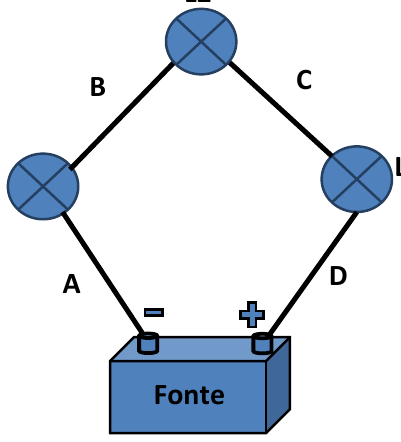
\includegraphics[width=0.95\linewidth]{static/simulados/coluni/figuras/2018/questao-23/figura-1.png}
\end{figure}
% COLUNI-AUTO-FIGURES-END

Os estudantes observaram o circuito construído conforme a figura acima, e constataram que as lâmpadas brilhavam. Ao explicar o funcionamento do circuito, afirmaram:

\par

Aline: As lâmpadas estão ligadas em série. Márcia: Se a lâmpada $L_1$ queimar, as lâmpadas $L_2$ e $L_3$ continuam acesas. Diego: Ligando os fios B e C, por um fio condutor, a lâmpada $L_2$ apagará. Samuel: Se a lâmpada $L_3$ queimar, nenhuma lâmpada acenderá.

\par

Após as discussões e explicações a respeito do funcionamento do circuito apresentado, concluiu-se que estão CORRETAS as afirmações feitas por:


\begin{enumerate}
\item Aline, Diego e Samuel.
\item Aline, Márcia e Samuel.
\item Márcia, Diego e Samuel.
\item Aline, Márcia e Diego.\end{enumerate}
